\documentclass{beamer}

\usetheme{Madrid}
\usecolortheme{default}

\usepackage{graphicx}
\usepackage{tikz}
\usetikzlibrary{shapes.geometric, arrows.meta, positioning}

% TikZ styling for the flowchart
\tikzstyle{process} = [
    rectangle,
    rounded corners,
    minimum width=3.5cm,
    minimum height=1cm,
    text centered,
    draw=blue!70,
    fill=blue!10,
    thick
]

\tikzstyle{arrow} = [
    thick,
    ->,
    >=stealth
]

\title{Robust End-to-End Automatic License Plate Recognition (ALPR)}
\author{Farhan Tanvir Utshaw}
\institute{Missouri State University}


\begin{document}

\frame{\titlepage}

% --------------------------------------------------
\begin{frame}{Motivation}
\begin{itemize}
    \item ALPR is widely used in security, parking systems, and tolling automation.
    \item Real-world images are degraded: blur, rotation, weather, illumination.
    \item Goal: Build an end-to-end ALPR system robust to \textbf{non-ideal images}.
    \item Dataset: Full CCPD2019 (base + blur + rotate + weather + challenge).
\end{itemize}
\end{frame}

% --------------------------------------------------
\begin{frame}{Dataset Overview}
\begin{itemize}
    \item CCPD2019: $\sim$250k images
    \item Subsets:
    \begin{itemize}
        \item \textbf{ccpd\_base} – clean images
        \item \textbf{ccpd\_blur} – motion blur, defocus
        \item \textbf{ccpd\_rotate} – rotated plates
        \item \textbf{ccpd\_tilt} – perspective distortion
        \item \textbf{ccpd\_weather} – rain, fog, low-light
        \item \textbf{ccpd\_challenge} – extremely hard cases
    \end{itemize}
    \item YOLO used to extract 140k plate crops
    \item Final OCR training set: mixture of clean + degraded crops
\end{itemize}
\end{frame}

\begin{frame}{Dataset Examples: Clean vs Degraded}

\textbf{Input to the YOLO}

\vspace{0.2cm}

\centering
% Setup for the 2x2 grid
\begin{figure}
    \begin{minipage}{0.48\textwidth}
        \centering
        % REPLACE WITH YOUR CLEAN IMAGE PATH
        \includegraphics[height=0.7\textheight,width=0.9\linewidth]{images/ccpd_base_example.jpg} 
        \caption {Base}
    \end{minipage}\hfill
    \begin{minipage}{0.48\textwidth}
        \centering
        % REPLACE WITH YOUR BLUR IMAGE PATH
        \includegraphics[height=0.7\textheight, width=0.9\linewidth]{images/ccpd_blur_example.jpg}
        \caption {Blur}
    \end{minipage}

    
\end{figure}
\end{frame}

\begin{frame}{Dataset Examples: Clean vs Degraded}
\textbf{Input to the YOLO}
\centering
\begin{figure}

\begin{minipage}{0.48\textwidth}
        \centering
        % REPLACE WITH YOUR ROTATED IMAGE PATH
        \includegraphics[height=0.4\textheight, width=0.9\linewidth]{images/ccpd_rotate_example.jpg}
        \caption {Rotation}
    \end{minipage}\hfill
    \begin{minipage}{0.48\textwidth}
        \centering
        % REPLACE WITH YOUR WEATHER IMAGE PATH
        \includegraphics[height=0.4\textheight, width=0.9\linewidth]{images/ccpd_weather_example.jpg}
        \caption {Weather}
    \end{minipage}

\end{figure}
\end{frame}



\begin{frame}{YOLO cropped license plate | Input to the CRNN}
\centering
\begin{figure}

\begin{minipage}{0.48\textwidth}
        \centering
        % REPLACE WITH YOUR ROTATED IMAGE PATH
        \includegraphics[height=0.4\textheight, width=0.9\linewidth]{images/l1.jpg}
    \end{minipage}\hfill
    \begin{minipage}{0.48\textwidth}
        \centering
        % REPLACE WITH YOUR WEATHER IMAGE PATH
        \includegraphics[height=0.4\textheight, width=0.9\linewidth]{images/l2.jpg}
    \end{minipage}

\end{figure}
\end{frame}


\begin{frame}{OCR Model: CRNN Architecture}

\textbf{CRNN Goal:} Convert the $128 \times 32$ Plate Image into a Variable-Length Text Sequence.


\begin{enumerate}
    \item \textbf{CNN (Feature Extraction)}
    \begin{itemize}
        \item \textbf{Role:} Extracts visual features (strokes, characters parts) from the 2D image.
        \item \textbf{Input:} Standardized Plate Crop ($128 \times 32$ Grayscale).
        \item \textbf{Output:} A 3D feature map tensor that is internally transformed into a sequence of vectors by collapsing the height dimension (Map-to-Sequence step). 
    \end{itemize}

    \item \textbf{Bi-Directional LSTM (Sequence Modeling)}
    \begin{itemize}
        \item \textbf{Role:} Processes the feature vectors sequentially from left-to-right and right-to-left.
        \item \textbf{Function:} Learns the contextual dependencies and potential language patterns of the license plate sequence.
        \item \textbf{Output:} A probability distribution over all characters (\texttt{0-9, A-Z, \dots}) and a special \texttt{<blank>} token for every time step (column).
    \end{itemize}

    
\end{enumerate}

\end{frame}


\begin{frame}{OCR Model: CRNN Architecture}
    \textbf{CRNN Goal:} Convert the $128 \times 32$ Plate Image into a Variable-Length Text Sequence.
    \begin{enumerate}
        \item \textbf{CTC (Connectionist Temporal Classification)}
    \begin{itemize}
        \item \textbf{Role:} Solves the crucial problem of alignment (mapping variable-length image features to fixed-length ground truth labels).
        \item \textbf{Function:} Collapses the redundant, per-time-step sequence (e.g., \texttt{C-C-C-<blank>-A-A}) by removing repeated characters and \texttt{<blank>} tokens.
        \item \textbf{Output:} The final, clean recognized license plate text (e.g., \texttt{C A}).
    \end{itemize}
    \end{enumerate}
\end{frame}


\begin{frame}{Phase\,1: Baseline Training on Clean CCPD Data}

\textbf{Objective:}
Train CRNN on high–quality, clean license plate crops to establish a strong baseline but it performed really well.

\vspace{0.3cm}

\textbf{Dataset Source:}
\begin{itemize}
    \item CCPD\_Base subset only (clean, centered, well-lit plates)
    \item Crops extracted using YOLOv8 detector
    \item Output folder: \texttt{crops/}
\end{itemize}

\vspace{0.25cm}

\textbf{Dataset Size:}
\begin{itemize}
    \item $\sim$200{,}000 good plate crops
    \item Minimal variation → ideal for OCR learning
\end{itemize}

\vspace{0.25cm}

\textbf{Result:}
\begin{itemize}
    \item CRNN achieves \textbf{near-perfect accuracy} on test set
    \item Excellent performance on clean plates
    \item \textbf{Weak robustness} to blur, rotation, tilt, weather, etc.
\end{itemize}

\end{frame}

\begin{frame}{Phase\,2: Robust Training on Mixed (Good + Bad) Data}

\textbf{Objective:}
Improve robustness by including challenging plates in the OCR training set.

\vspace{0.3cm}

\textbf{Bad Subsets Used:}
\begin{itemize}
    \item \texttt{ccpd\_blur}, \texttt{ccpd\_rotate}, \texttt{ccpd\_tilt}
    \item \texttt{ccpd\_weather}, \texttt{ccpd\_challenge}
\end{itemize}

\vspace{0.25cm}

\textbf{Dataset Construction:}
\begin{itemize}
    \item Crops extracted via YOLO from all “bad” subsets  
    → \textbf{119,766 challenging crops}
    \item Plus a balanced sample of \textbf{20,000 clean crops}
    \item Combined into: \texttt{crops\_mix/}
\end{itemize}

\vspace{0.25cm}

\textbf{Advantages:}
\begin{itemize}
    \item CRNN exposed to diverse distortions
    \item Improved generalization to real-world conditions
    \item Significantly more robust detections
\end{itemize}

\end{frame}


% --------------------------------------------------
\begin{frame}{Pipeline Overview (Theory)}
\centering
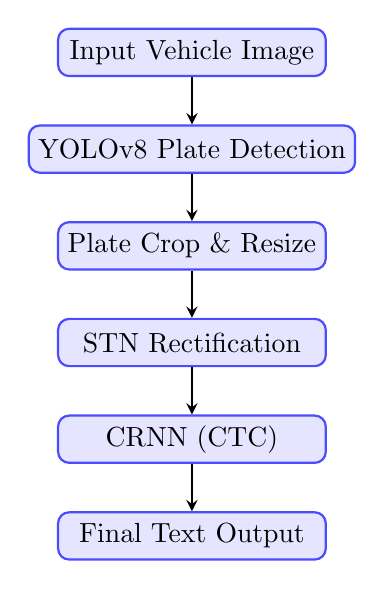
\begin{tikzpicture}[node distance=0.6cm]

\tikzstyle{process} = [
    rectangle,
    rounded corners,
    minimum width=3.4cm,
    minimum height=0.6cm,
    text centered,
    draw=blue!70,
    fill=blue!10,
    thick
]

\node (input)   [process] {Input Vehicle Image};
\node (detector)[process, below=of input] {YOLOv8 Plate Detection};
\node (crop)    [process, below=of detector] {Plate Crop \& Resize};
\node (rect)    [process, below=of crop] {STN Rectification};
\node (ocr)     [process, below=of rect] {CRNN (CTC)};
\node (output)  [process, below=of ocr]  {Final Text Output};

\draw[arrow] (input) -- (detector);
\draw[arrow] (detector) -- (crop);
\draw[arrow] (crop) -- (rect);
\draw[arrow] (rect) -- (ocr);
\draw[arrow] (ocr) -- (output);

\end{tikzpicture}
\end{frame}

\begin{frame}{Methodology Overview}

\begin{enumerate}
    \item \textbf{YOLOv8 License Plate Detection}  
        Trained a detector on CCPD to localize plates in all images.

    \item \textbf{Plate Crop Extraction}  
        Used the trained YOLO model to generate standardized $128 \times 32$ grayscale crops.

    \item \textbf{OCR Model Training (Two-Phase)}  
        \begin{itemize}
            \item Phase\,1: CRNN trained on clean CCPD\_Base crops.
            \item Phase\,2: CRNN retrained on mixed robust dataset
                  (clean + blurred + rotated + weather-distorted plates).
        \end{itemize}

    \item \textbf{End-to-End Inference Pipeline}  
        YOLO → Crop → Optional STN → CRNN decoding.
\end{enumerate}

\end{frame}

\begin{frame}{License Plate Detection with YOLOv8}

\textbf{Goal:} Accurately detect plate bounding boxes across all CCPD subsets.

\vspace{0.25cm}

\textbf{Steps:}
\begin{itemize}
    \item Trained YOLOv8 on CCPD labels (train/val split).
    \item Achieved reliable detection even under blur, tilt, rotation, occlusion.
    \item Used trained model to crop $>140{,}000$ plates from all CCPD subsets.
\end{itemize}

\vspace{0.3cm}

\textbf{Detection Output:}
\begin{itemize}
    \item Bounding box selection (highest confidence)
    \item Tight crop
    \item Resized to $128 \times 32$ grayscale for OCR
\end{itemize}

\end{frame}

\begin{frame}{OCR Training: Phase\,2 (Robust Mixed Dataset)}

\textbf{Mixed Dataset Construction:}
\begin{itemize}
    \item 119{,}766 challenging crops from:
          blur / rotate / tilt / weather / challenge subsets.
    \item 20{,}000 clean CCPD\_Base crops (balanced sampling).
    \item Total = 139{,}766 images in \texttt{crops\_mix/}.
\end{itemize}

\vspace{0.25cm}

\textbf{Training Result:}
\begin{itemize}
    \item Converged stable model with 
          \textbf{Best Validation Loss: 0.0331}.
    \item Significantly better recognition on noisy images.
    \item Improved generalization to real car photos.
\end{itemize}

\end{frame}



% --------------------------------------------------
\begin{frame}{YOLO Plate Detection}
\begin{itemize}
    \item Trained YOLOv8n on 200k CCPD images.
    \item Achieved:
    \begin{itemize}
        \item Precision: 1.00
        \item Recall: 1.00
        \item mAP50: 0.995
    \end{itemize}
    \item Detector successfully used to crop plates from \textbf{all other CCPD subsets}.
\end{itemize}
\end{frame}

% --------------------------------------------------
\begin{frame}{OCR Model: CRNN (Baseline)}
\begin{itemize}
    \item CNN $\to$ BiLSTM $\to$ CTC decoding
    \item Inputs: 128 × 32 grayscale crops
    \item Initial training on clean CCPD crops gave:
    \begin{itemize}
        \item Train accuracy: 100\%
        \item Test accuracy: 100\% (on base)
    \end{itemize}
    \item Poor robustness on blurred/tilted/rotated plates → motivates STN + heavy augmentation.
\end{itemize}
\end{frame}

% --------------------------------------------------
\begin{frame}{OCR Model: STN-CRNN (Robust Version)}
\begin{itemize}
    \item Spatial Transformer Network performs:
    \begin{itemize}
        \item geometric correction,
        \item de-tilting,
        \item mild de-blurring (affine stabilizing).
    \end{itemize}
    \item Combined with CRNN improves robustness.
    \item Trained on:
    \begin{itemize}
        \item 20k clean plates
        \item 100k+ degraded plates (blur, rotate, weather)
    \end{itemize}
\end{itemize}
\end{frame}

% --------------------------------------------------



% --------------------EVALUATION------------------------------

\begin{frame}{Evaluation: CRNN vs.\ STN--CRNN}

\textbf{Evaluation Setup}
\begin{itemize}
    \item Held-out CCPD subset of \textbf{1000 plate crops} (not used in training).
    \item Goal: measure robustness on mixed-quality images (blur/tilt/weather/rotate).
    \item STN attempts to \textbf{geometrically rectify} plates before recognition.
\end{itemize}

\vspace{0.3cm}

\begin{table}[h!]
\centering
\renewcommand{\arraystretch}{1.3}
\begin{tabular}{|c|c|c|}
\hline
\textbf{Model} & \textbf{Correct / 1000} & \textbf{Accuracy} \\
\hline
CRNN\_v2 (no STN) & 991 / 1000 & 0.9910 \\
\hline
STN + CRNN\_v2 & 981 / 1000 & 0.9810 \\
\hline
\end{tabular}
\end{table}

\vspace{0.3cm}

\textit{Observation:} In this dataset split, the vanilla CRNN slightly outperforms the STN variant.  
STN helps mainly on severe geometric distortions, but may reduce performance on already-normalized crops.

\end{frame}












% -------------------ALPR Inference Pipeline-------------------------------
\begin{frame}{End-to-End ALPR Inference Pipeline (v2)}

\centering
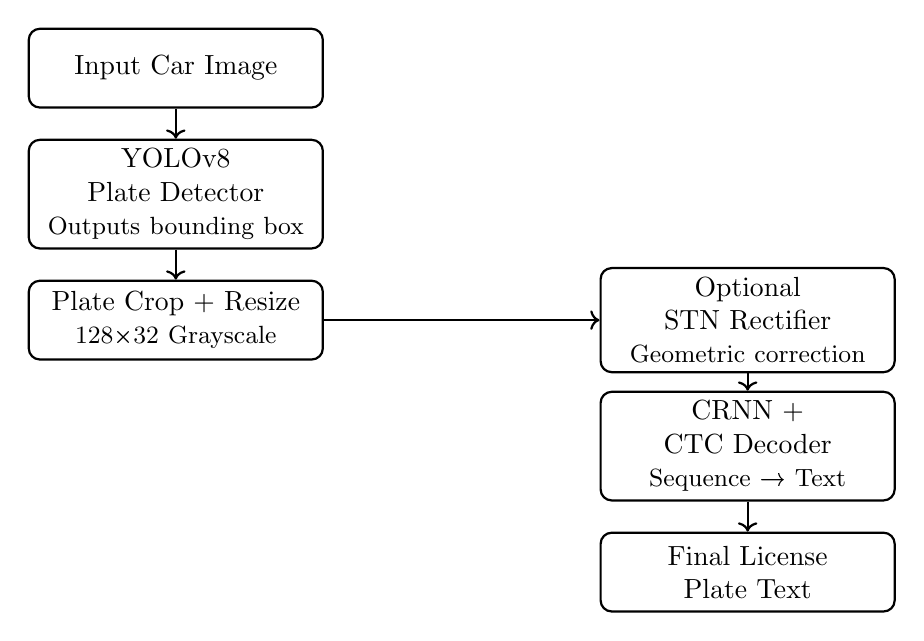
\begin{tikzpicture}[
    node distance=1.6cm,
    box/.style={
        rectangle,
        draw,
        rounded corners,
        align=center,
        text width=3.5cm,
        minimum height=1cm,
        thick
    },
    arrow/.style={->, thick}
]

% Left Column
\node[box] (input) {Input Car Image};
\node[box, below of=input] (yolo) {YOLOv8 Plate Detector\\\small Outputs bounding box};
\node[box, below of=yolo] (crop) {Plate Crop + Resize\\\small 128×32 Grayscale};

% Right Column (shifted to avoid overflow)
\node[box, right=3.5cm of crop] (stn) {Optional STN Rectifier\\\small Geometric correction};
\node[box, below of=stn] (crnn) {CRNN + CTC Decoder\\\small Sequence → Text};
\node[box, below of=crnn] (output) {Final License Plate Text};

% Arrows (L→R)
\draw[arrow] (input) -- (yolo);
\draw[arrow] (yolo) -- (crop);
\draw[arrow] (crop) -- (stn);
\draw[arrow] (stn) -- (crnn);
\draw[arrow] (crnn) -- (output);

\end{tikzpicture}

\end{frame}





% -------------------CONCLUSION-------------------------------
\begin{frame}{Conclusion}
\begin{itemize}
    \item Completed robust ALPR pipeline:
    \begin{itemize}
        \item YOLOv8 detector
        \item CRNN OCR
        \item STN-based geometric rectification
    \end{itemize}
    \item Robust performance even on degraded CCPD subsets.
\end{itemize}
\end{frame}

% --------------------------------------------------
\begin{frame}{Q \& A}
\centering
\Huge Thank You!
\end{frame}

\end{document}
